\section{Use Cases}

\subsection{Actors}
An actor specifies a role to be played by internal or external persons interacting with the application. In our case, we have only one actor, namely the end-user. The user is a person who does not necessarily have much education in using our application, but will use it regularly in his workday. 

\subsection{Use case diagrams}
For a combined figure of all the use cases, see figure \ref{fig:usecase} below.

\begin{figure}[h!]
\begin{center}
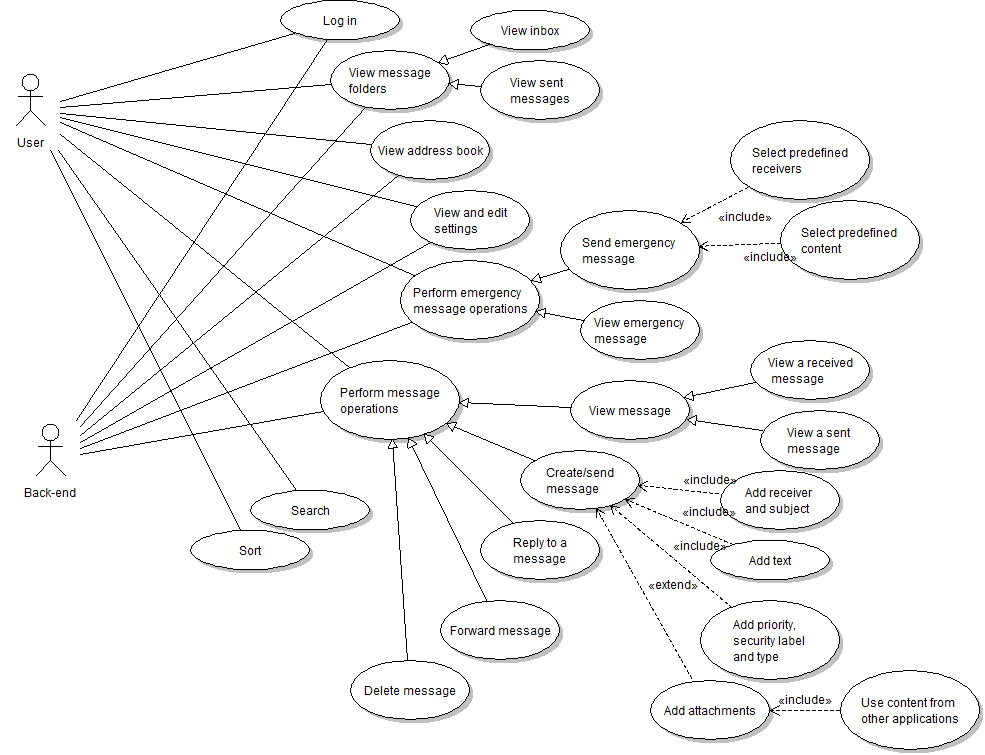
\includegraphics[width=\textwidth]{kpro-use-case}
\caption{Use case diagram} \label{fig:usecase}
\end{center}
\end{figure}

\subsection{Textual use cases}
Each of the use cases is described below, so that the use case diagram will be easier to understand. See table \ref{tab:viewmessages} - \ref{tab:settings} from page \pageref{tab:viewmessages} to \pageref{tab:settings} for a more detailed explanation of the use cases.

\begin{table}
\begin{center}
\begin{center}
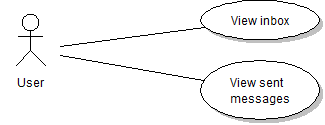
\includegraphics[width=\textwidth]{view_messages}
\end{center}
\begin{tabular}{p{3cm}|p{12cm}}\hline
\textbf{Element} & \textbf{Description} \\ \hline \hline
Use case name & View messages \\
Requirement & FR3, FR4 \\
Goal & View received and sent messages \\
Summary &The user would like to view received and sent messages \\ \hline
Preconditions &
\begin{enumerate}
\item{}The application is running
\item{}The user is logged in
\end{enumerate} \\ \hline
Flow of Events &
\begin{enumerate}
\item{}The user selects a message from either the inbox or sent messages
\item{}Message is showed to user
\end{enumerate} \\ \hline
Exceptions & There are no existing messages\\ \hline
\end{tabular}
\end{center}
\caption{Textual use case - View messages} \label{tab:viewmessages}
\end{table}

\begin{table}
\begin{center}
\begin{center}
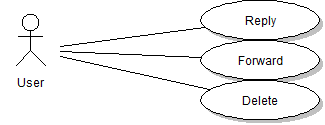
\includegraphics[width=\textwidth]{reply_forward_delete}
\end{center}
\begin{tabular}{p{3cm}|p{12cm}} \hline
\textbf{Element} & \textbf{Description} \\ \hline \hline
Use case name & Reply, forward and delete \\
Requirement & FR8	 \\
Goal & Reply, forward and delete messages\\
Summary & The user would like to reply to a message, forward it or delete it \\ \hline
Preconditions &
\begin{enumerate}
\item{}The application is running
\item{}The user is logged in
\end{enumerate} \\ \hline
Flow of Events &
\begin{enumerate}
\item{}The user selects a message from either the sent or inbox messages
\item{}Message is showed to user
\item{}User chooses to reply, forward or delete the message
\end{enumerate} \\ \hline
Exceptions & There are no existing messages\\ \hline
\end{tabular}
\end{center}
\caption{Textual use case - Reply, forward and delete message} \label{tab:reply}
\end{table}

\begin{table}
\begin{center}
\begin{center}
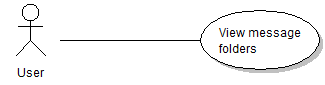
\includegraphics[width=\textwidth]{view_message_folders}
\end{center}
\begin{tabular}{p{3cm}|p{12cm}} \hline
\textbf{Element} & \textbf{Description} \\ \hline \hline
Use case name & View message folders \\ 
Requirement & FR3, FR4 \\
Goal & View inbox and sent messages \\ 
Summary &The user would like to view the inbox and a list of sent messages \\ \hline
Preconditions &
\begin{enumerate}
\item{}The application is running
\item{}The user is logged in
\end{enumerate} \\ \hline
Flow of Events &
\begin{enumerate}
\item{}The user enters the inbox or sent messages
\item{}The list of messages in the inbox or sent messages is presented to the user
\end{enumerate} \\ \hline
Exceptions & There are no existing messages\\ \hline
\end{tabular}
\end{center}
\caption{Textual use case - View message} \label{tab:viewmessagefolders}
\end{table}

\begin{table}
\begin{center}
\begin{center}
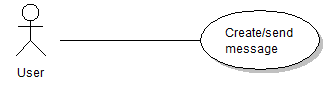
\includegraphics[width=\textwidth]{create_message}
\end{center}
\begin{tabular}{p{3cm}|p{12cm}} \hline
\textbf{Element} & \textbf{Description} \\ \hline \hline
Use case name & Create message \\
Requirement & FR2, FR6 \\
Goal & User creates and sends a complete message \\ \hline
Summary &The user would like to create/send a message to a receiver with a subject and text. The user would also like to set the priority, security label and type of the message as well as being able to add an attachment from other applications. \\ \hline
Preconditions &
\begin{enumerate}
\item{}The application is running
\item{}The user is logged in
\end{enumerate} \\ \hline
Flow of Events &
\begin{enumerate}
\item{}User selects new message
\item{}The user adds the recipient(s) and subject to the message
\item{}The user sets the priority, security label and type
\item{}The user adds attachments if needed
\end{enumerate} \\ \hline
Exceptions & The user does not set priority, security label and type and default values are set\\ \hline
\end{tabular}
\end{center}
\caption{Textual use case - Create message} \label{tab:createmessage}
\end{table}

\begin{table}
\begin{center}
\begin{center}
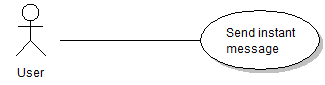
\includegraphics[width=\textwidth]{send_instant_message}
\end{center}
\begin{tabular}{p{3cm}|p{12cm}} \hline
\textbf{Element} & \textbf{Description} \\ \hline \hline
Use case name & Send instant message \\
Requirement & FR9 \\
Goal & User sends an instant message \\ \hline
Summary & The user sends an instant message with predefined content to predefined receivers \\ \hline
Preconditions &
\begin{enumerate}
\item{}The application is running
\item{}The user is logged in
\end{enumerate} \\ \hline
Flow of Events &
\begin{enumerate}
\item{}User selects new instant message
\item{}The user sends the message
\end{enumerate} \\ \hline
Exceptions & The predefined values have not been set\\ \hline
\end{tabular}
\end{center}
\caption{Textual use case - Send instant message} \label{tab:createmessage}
\end{table}

\begin{table}
\begin{center}
\begin{center}
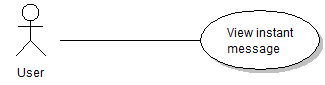
\includegraphics[width=\textwidth]{view_instant_message}
\end{center}
\begin{tabular}{p{3cm}|p{12cm}} \hline
Element & Description \\ \hline \hline
Use case name & View high priority message \\
Requirement & FR12 \\
Goal & User views a high priority message \\
Summary & The user receives and views a high priority message \\ \hline
Preconditions &
\begin{enumerate}
\item{}The application is running
\item{}The user is logged in
\end{enumerate} \\ \hline
Flow of Events &
\begin{enumerate}
\item{}User receives a high priority message
\item{}A popup appear on the users screen
\item{}User presses the popup and views the high priority message
\end{enumerate} \\ \hline
Exceptions & - \\ \hline
\end{tabular}
\end{center}
\caption{Textual use case - View instant message} \label{tab:createmessage}
\end{table}

\begin{table}
\begin{center}
\begin{center}
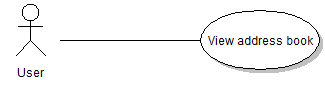
\includegraphics[width=\textwidth]{view_address_book}
\end{center}
\begin{tabular}{p{3cm}|p{12cm}} \hline
\textbf{Element} & \textbf{Description} \\ \hline \hline
Use case name & View the address book \\
Requirement & FR5 \\
Goal & User can view and interact with the address book \\
Summary &The user enters the address book and is able to view  contacts \\ \hline
Preconditions &
\begin{enumerate}
\item{}The application is running
\item{}The user is logged in
\end{enumerate} \\ \hline
Flow of Events &
\begin{enumerate}
\item{}User selects address book
\item{}User selects a contact to send a message to
\end{enumerate} \\ \hline
Exceptions & - \\ \hline
\end{tabular}
\end{center}
\caption{Textual use case - View the address book} \label{tab:viewandinteract}
\end{table}

\begin{table}
\begin{center}
\begin{center}
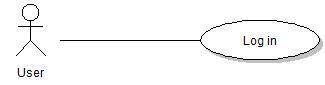
\includegraphics[width=\textwidth]{login}
\end{center}
\begin{tabular}{p{3cm}|p{12cm}} \hline
\textbf{Element} & \textbf{Description} \\ \hline \hline
Use case name & Log in \\ 
Requirement & FR1 \\
Goal & User logs in with a username and password \\ \hline
Summary &The user is prompted with a login screen and must type in his username and password \\hline
Preconditions &
\begin{enumerate}
\item{}The application is running
\end{enumerate} \\ \hline
Flow of Events &
\begin{enumerate}
\item{}User starts application
\item{}User is prompted with username and password
\item{}User types in username and password and presses the login button
\item{}User gains access to the application data and functionality
\end{enumerate} \\ \hline
Exceptions & User types wrong username and password and is denied access \\ \hline
\end{tabular}
\end{center}
\caption{Textual use case - Log in} \label{tab:login}
\end{table}

\begin{table}
\begin{center}
\begin{center}
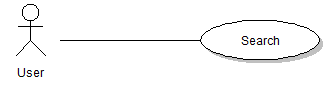
\includegraphics[width=\textwidth]{search}
\end{center}
\begin{tabular}{p{3cm}|p{12cm}} \hline
\textbf{Element} & \textbf{Description} \\ \hline \hline
Use case name & Search \\
Requirement & FR14 \\
Goal & User receives search results for a given search text \\ \hline
Summary & The user search in the application for messages, contacts etc through a search field at the top of the screen \\ \hline
Preconditions &
\begin{enumerate}
\item{}The application is running
\item{}The user is logged in
\end{enumerate} \\ \hline
Flow of Events &
\begin{enumerate}
\item{}User highlights search field and inserts his the text he wants to search for
\item{}User presses the search button
\item{}Application shows search results to the user
\end{enumerate}\\ \hline
Exceptions & - \\ \hline
\end{tabular}
\end{center}
\caption{Textual use case - Search} \label{tab:search}
\end{table}

\begin{table}
\begin{center}
\begin{center}
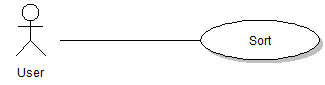
\includegraphics[width=\textwidth]{sort}
\end{center}
\begin{tabular}{p{3cm}|p{12cm}} \hline
\textbf{Element} & \textbf{Description} \\ \hline \hline
Use case name & Sort \\
Requirement & FR13 \\
Goal & User sorts the messages in his inbox \\ \hline
Summary & The user chosoes a value that he wishes the messages to be sorted by \\ \hline
Preconditions &
\begin{enumerate}
\item{}The application is running
\item{}The user is logged in
\item{}There are messages to sort
\end{enumerate} \\ \hline
Flow of Events &
\begin{enumerate}
\item{}The user selects the value he wishes the messages to be sorted by
\item{}The application sorts the messages and displays them to the user
\end{enumerate} \\ \hline
Exceptions & - \\ \hline
\end{tabular}
\end{center}
\caption{Textual use case - Sort} \label{tab:search}
\end{table}

\begin{table}
\begin{center}
\begin{center}
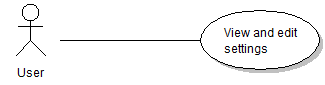
\includegraphics[width=\textwidth]{settings}
\end{center}
\begin{tabular}{p{3cm}|p{12cm}} \hline
\textbf{Element} & \textbf{Description} \\ \hline \hline
Use case name & Settings \\ 
Requirement & FR10 \\
Goal & The user can alter settings \\ \hline
Summary & The user enters the settings menu and alter the settings to suit his own preferences \\ \hline
Preconditions &
\begin{enumerate}
\item{}The application is running
\item{}The user is logged in
\end{enumerate} \\ \hline
Flow of Events &
\begin{enumerate}
\item{}User presses the settings button
\item{}User alters the settings he wishes to
\item{}Application saves the alterations
\end{enumerate} \\ \hline
Exceptions & - \\ \hline
\end{tabular}
\end{center}
\caption{Textual use case - View and edit settings} \label{tab:settings}
\end{table}
